\documentclass[tikz,border=12pt]{standalone}
\usepackage[T1]{fontenc}
\usepackage{mathpazo}
\usepackage{amsmath,amssymb}
\usepackage{pgfplots}
\pgfplotsset{compat=1.18}

\definecolor{stblue}{HTML}{7B97AD}
\definecolor{rwgold}{HTML}{B8995E}
\definecolor{sage}{HTML}{7A9A7E}
\definecolor{dkbrown}{HTML}{3D3530}
\definecolor{wmgray}{HTML}{7B7067}
\definecolor{cream}{HTML}{F9F6F0}
\definecolor{border}{HTML}{D4C9B8}
\definecolor{terracotta}{HTML}{C47A6A}
\definecolor{lavender}{HTML}{907EA0}

\begin{document}
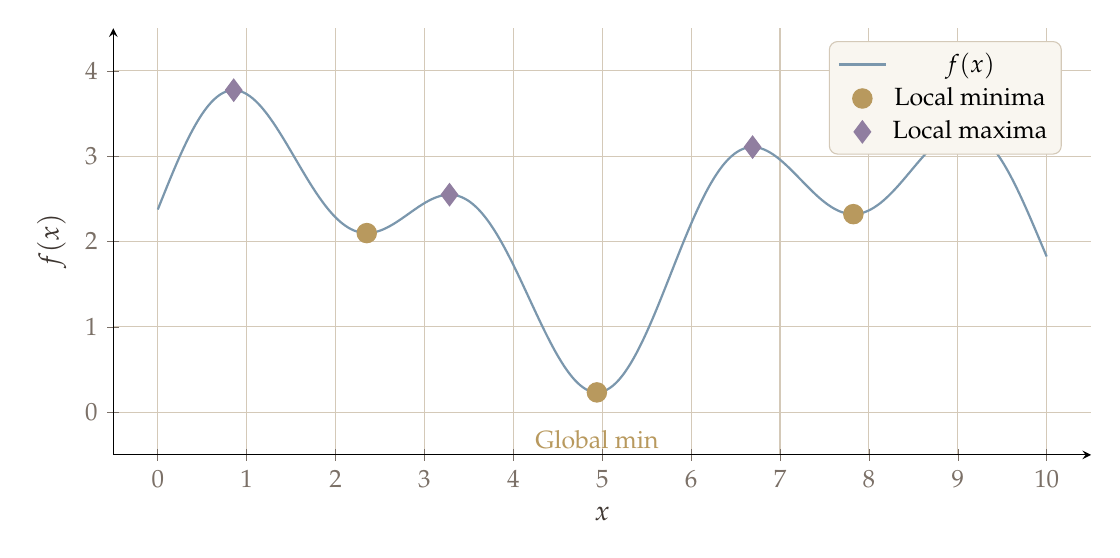
\begin{tikzpicture}
\begin{axis}[
  width=14cm, height=7cm,
  axis lines=left,
  xlabel={$x$}, ylabel={$f(x)$},
  every axis label/.style={font=\normalsize, color=dkbrown},
  every tick label/.style={font=\small, color=wmgray},
  grid=major,
  grid style={border, thin},
  tick style={wmgray},
  xmin=-0.5, xmax=10.5,
  ymin=-0.5, ymax=4.5,
  legend pos=north east,
  legend style={font=\small, fill=cream, draw=border, rounded corners=3pt},
]

% Function: f(x) = sin(x) + 0.8*sin(2.2*x) + 0.015*(x-5)^2 + 2
\addplot[stblue, thick, smooth, domain=0:10, samples=300]
  {sin(deg(x)) + 0.8*sin(deg(2.2*x)) + 0.015*(x-5)^2 + 2};
\addlegendentry{$f(x)$}

% Local minima — coordinates computed from the actual function
\addplot[only marks, mark=*, mark size=3.5pt, rwgold, mark options={fill=rwgold}]
  coordinates {(2.351,2.099) (4.940,0.232) (7.825,2.321)};
\addlegendentry{Local minima}

% Local maxima — coordinates computed from the actual function
\addplot[only marks, mark=diamond*, mark size=4pt, lavender, mark options={fill=lavender}]
  coordinates {(0.854,3.774) (3.282,2.549) (6.691,3.107) (9.064,3.311)};
\addlegendentry{Local maxima}

% Global min label
\node[rwgold, font=\small, anchor=north] at (axis cs:4.940,-0.1) {Global min};

\end{axis}
\end{tikzpicture}
\end{document}
